\documentclass[12pt]{article}
\usepackage{nips15submit_e,times}
\usepackage{url,graphicx,tabularx,array,geometry,amsmath,amssymb,amsthm,lipsum,hyperref,dsfont}

\newcommand{\unionf}{\bigcup_{n=1}^{\infty} \mathcal{F}_n}
\newcommand{\F}{\mathcal{F}}
\newcommand{\E}{\mathbb{E}}
\newcommand{\PP}{\mathbb{P}}
\newcommand{\Hi}{\mathcal{H}}
\newcommand{\A}{\mathcal{A}}
\newcommand{\Aseq}{\{A_k\}_{k=1}^{\infty}}
\newcommand{\unionA}{\bigcup_{k=1}^{\infty} A_k}
\newcommand{\argmax}{\operatornamewithlimits{argmax}}

\nipsfinalcopy

\begin{document}

\title{CS181P Final Project Proposal \#2}

\author{
Santi Santichaivekin, Jingyi Liu, Jacob Boerma, Lorraine Zhao, Princewill Okoroafor\\
Harvey Mudd College and Claremont McKenna College\\
Claremont, California, USA\\
}

\maketitle

\section{Team}
The team includes Santi Santichaivekin,
Jingyi Liu,
Jacob Boerma,
Lorraine Zhao, and 
Princewill Okoroafor.
The team name is Go Pika Pika!
The team logo is provided below.


\includegraphics[width=0.25\textwidth]{../Logo/logo1.jpg}

\section{Project}

We will attempt the second project listed on the project ideas:
\begin{quote}
ML, Search, and Compression. It has been shown that ML is a form of search (we will see this during the course, for example in Montan\~ez (Chapter 3)), and also shown that ML can be viewed as a form of compression (as in minimum description length approaches). Can we show compression is a form of search, search a form of compression, search a form of ML, or compression a form of ML, to make a triangle of two-way equivalences? Or taking a subset of these equivalences, can we apply a set of results from one domain to the other, such as forming no free lunch theorems for compression?
\end{quote}
We hypothesize that all the three problems can be phrased as one another. If we prove the three-way equivalency among the three problems, then we can apply different theories from one field to another.
Also, this problem is applicable to the real world, where we can solve actual real world problems by directing them as either ML, search, or compression. 

\section{Initial Plan of Attack}

We will start with understanding the concepts of ML, data compression, and search individually, and then trying to prove the “No Free Lunch” theorem for data compression among other theorems of search that might be applied to data compression. We can then look for algorithms for data compression and obtain insights about how it might be framed as a machine learning problem and search.

\section{Separation of Work}

For now, we will each read the papers and get on the same level of understanding. Once we have a good understanding of ML, compression, and search, we might split up work based on sub-problems that appear. We have divided the readings to different team members, so that one person can focus on one or two readings, and then update the rest of the team members on what he/she learned.

\begin{itemize}
\item
Jacob will read about No Free Lunch on a high level, and will try to understand the Famine of Forte paper and how we might apply the same concepts to compression schemes.
\item
Santi will be trying to understand the No Free Lunch Theory and apply it to compression.
\item
Lorraine will go over her part of the readings and get a better understanding of Machine Learning and Searches, and try to link the two by establishing an equivalent relationship.
\item
Rose will be reading about data compression algorithms and see how to generalize them as search problems. 
\item
Princewill will also be reading about data compression algorithms and how they can be generalized as search problems. 
\end{itemize}

\section{Literature Review}

We have found some papers and textbooks that will be useful for our research.
We will read the suggested readings for the next few lectures in class, as well as the following papers/articles.

\newpage

\subsection*{Why ML Works} 

\url{http://www.cs.cmu.edu/~gmontane/montanez_dissertation.pdf} [Lorraine]

\newpage


\subsection*{Famine of Forte} 

\url{https://arxiv.org/pdf/1609.08913.pdf} [Jacob]

This paper uses a search framework to prove several bounds concerning the proportion of good problems for a search algorithm. 

The paper uses a finite \textbf{search space} $\Omega$, and objective is to find an element of the \textbf{target set} $T \subset \Omega$. Given an order of the search space $\Omega$, we can represent $T$ as a binary vector of size $\Omega$, because each element of the search space corresponds to one index in our vector. This vector is the \textbf{target function}. 

Finally, the paper describes an information resource $F$. Similar to the No Free Lunch for Optimization paper, Famine of Forte treats $F$ as an oracle from which our algorithm gets all information about a particular point $\omega \in \Omega$. $F(\omega)$ is the evaluation of $\omega$. Interestingly, this paper abstracts this resource as a finite bit string. 

Given a search space $\Omega$, a target set $T$, and an information resource $F$, a search problem is defined as $(\Omega, F, T)$. Since we are abstracting $F$ and $T$ to be finite-length bit strings, we can do lots of fun things!

The paper describes a \textbf{Black-box Search Algorithm}, that attempts to find points $\omega$ in the target set $T$. The algorithm keeps track of its history $H$, which is a series of tuples $h_i = (\omega_i, F(\omega_i))$. Each tuple keeps track of the ith call to the oracle. At iteration $i$, the algorithm uses the history up to this point to compute a distribution $P_i$ over $\Omega$. The algorithm chooses some element $w_i$ according to the distribution and consults the oracle. Note especially that this algorithm will perform queries $i_{\text{max}}$ times - only after does it check if we have seen a target element.

\begin{center}
    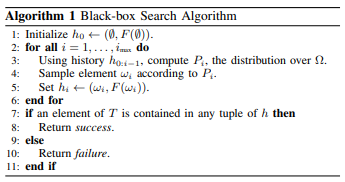
\includegraphics{FamineForte/BlackBoxAlgo.PNG}
\end{center}

We care about the performance of our search algorithm, since it is sufficiently general to represent many ML algorithms. 

Since the algorithm performs $i_{\text{max}}$ queries to the oracle, but this number can change, we may measure its performance by the expected per-query probability of success $q(T|F)$. The paper goes on to discuss how since this expectation is over all sources of randomness, it is equal to the probability of success for samples drawn from an appropriately averaged distribution - I don't really understand this. 

\begin{center}
    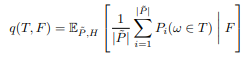
\includegraphics{FamineForte/ExpectedSuccess.PNG}
\end{center}

The paper defines $p(T,F)$ to be the expected probability of success when performing uniform random sampling, and uses this a baseline for the performance of our algorithm. It may be worth checking out the following paper, since it is referenced by Famine of Forte when discussion $p(T,F)$. 


W. Dembski and R. Marks II, “Conservation of information in search:
Measuring the cost of success,” Systems, Man and Cybernetics, Part A:
Systems and Humans, IEEE Transactions on, vol. 39, no. 5, pp. 1051
–1061, sept. 2009

\textbf{Theorem 1.} Famine of Forte

This result shows that the proportion of search problems with performance $q(T,F) \geq q_{\text{min}}$ is bounded above. Formally, the paper defined a set $\tau_k$, which is a set of k-hot target vectors. That is, $\tau_k$ contains all possible k-element target sets. 

The paper restricts the potential information resources to be in the set $B_m$, where $B_m$ is any set of binary strings such that each string has length $m$ or less. The paper then defines sets $R$ and $R_{q_{min}}$, where $R$ contains all search problems with k-length target sets, and $R_{q_{min}}$ those problems that perform as well as $q_{min}$. Their definitions are below: 
\begin{align*}
    \tau_k &= \{T | T \subset Q, |T| = k \in \mathds{N}\} \\ 
    R &= \{(T,F) | T \in \tau_k, F \in B_m\} \\
    R_{q_{min}} &= \{(T,F) | T \in \tau_k, F \in B_m, q(T,F) \geq q_{min}\}
\end{align*}
Then 
\begin{align*}
    \frac{|R_{q_{min}}|}{|R|} \leq \frac{p}{q_{min}} = \frac{k / |\Omega|}{q_{min}}
\end{align*}
The same result holds as $m \to \infty$ - as the size of the information sets grows.

Essentially, we are given a search space $\Omega$. In that space, the proportion of problems $(\Omega, F, T)$ in which our algorithm performs as well as $q_{min}$ is bounded above by an exact quantity. 

\bigskip 

\textbf{Corollary 1.} (Conservation of Active Information of Expectations)

If we define $I_{q(T,F)} = - \log(p/q(T,F))$, and effectively use this metric as our performance (with minimum performance $b$), then we get the result 

\[\frac{|R_b|}{|R|} \leq 2^{-b}\]

This uses the exact same set construction as theorem 1. Note that $I_{q(T,F)}$ looks very similar to the difference in surprisals of $p$ and $q$ - $p$ and $q$ are expected per-query probabilities of success. Our algorithm does better than uniform random sampling if $I$ is large, since that indicates a higher per-query probability of success. Thus the proportion of problems that do as well as $b$ under this metric is bounded above by $2^{-b}$. The paper discusses how this shows that the improved search method is equivalent to a uniform random sampler on a reduced search space. (I'm not really sure how this works) 

\bigskip

\textbf{Theorem 2.} Famine of Favorable Strategies
\begin{center}
    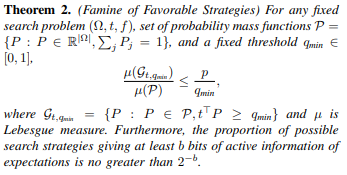
\includegraphics{FamineForte/FamineStrategy.PNG}
\end{center}

To be honest, I am not sure what this theorem is saying at the moment. My guess is that over all possible sequences $\{P_i\}_i$ of probabilities we can bound the number of algorithms that perform well on a given search problem. 

The paper discusses below how this places bounds on the number of favorable strategies on a given problem. This result and theorem 1 show that favorable problems for strategies and favorable strategies for problems are rare. 

\bigskip

\textbf{Theorem 3.} Success Under Dependence
\begin{center}
    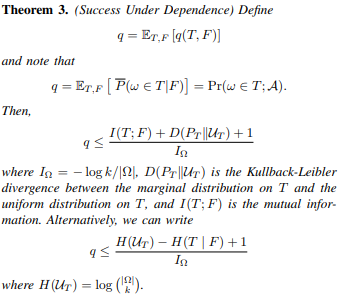
\includegraphics{FamineForte/SuccessUnderDependence.PNG}
\end{center}

This upper-bounds the expected performance of our algorithm on a search problem. The paper discusses how this bounds improves monotonically with the dependence between between our target set and information resources. That is, if our information is somewhat accurate, we can perform better! 

Other than that statement, I am having a hard time understanding this theorem. 


\bigskip

The paper then goes on to discuss examples of problems that fit under the framework, and proves theorem $1$ for the space of hyperparameters for a given algorithm $A$. It then shows that there cannot be a fitness function (information resource) that works well for all target sets in a search space. In other words, there is no One-Size-Fits-All fitness function. 

\bigskip

The paper then discusses why novel machine learning algorithms keep getting generated. Since the proportion of favorable strategies for a given problem is small and the proportion of favorable problems for a strategy is small, we must keep generating new strategies to deal with new problems.  

\subsubsection*{Further Reading} 

J. Culberson, “On the futility of blind search: An algorithmic view of
‘no free lunch’,” Evolutionary Computation, vol. 6, no. 2, pp. 109–127,
1998

** Just want to see no free lunch in another context

\bigskip

Compression and machine learning: a new perspective on feature space vectors

https://ieeexplore.ieee.org/abstract/document/1607268

** Compression - ML direction. 


\bigskip

An Introduction to Kolmogorov Complexity and Its Applications - skim chapters 2 and 3

** I read some stuff on Kolmogorov complexity, which is a way of measuring how random a string is / how hard a string is to generate. The complexity of a string is the number of characters needed to specify it (can use a programming language, so long as we include the specification in our length). Some strings are hard to generate, others are easy. There seems to already be a no-free-lunch theorem for compression based on the pigeonhold principle, but Kolmogorov complexity might help to give bounds on the number of strings that can be greatly compressed in a given language. 

\newpage

\subsection*{“Probabilistic machine learning and artificial intelligence”}
\url{https://www.nature.com/articles/nature14541} [Rose]

In his paper “Probabilistic machine learning and artificial intelligence”, Ghahramani provides an
overview of the probabilistic approach to machine learning and the state-of-art advances in
this field. Specifically, he explores five areas that fall under this framework including
probabilistic programming, Bayesian optimization, probabilistic data compression, automatic
model discovery, and hierarchical modeling. Under the framework of probabilistic modeling,
Ghahramani views machine learning as a process of inferring the most plausible model from a
given data set, which is in turn used to improve performance on future predictions. He points
out the advantages of using a probabilistic framework by arguing the central role of uncertainty
in machine learning models and identifies three sources of uncertainty that are typically present
in modeling (452-453). The uncertainties consist of the measurement noise of the data set, the
unknown parameters in a given model, and uncertainties about the general structure of the
mode. Thus probabilistic modeling comes as a natural remedy for dealing with various sources
of uncertainties and identifies the best model in accordance with data. Aside from its ability to
represent uncertainties in the model, probabilistic modeling also brings the advantage of
flexibility through the use of Bayesian non-parametric models, which grow in complexity as the
data set grows (454). Such flexibility allows machine learning models to capture the regularities
of the data and have better performance. Interestingly, he points out that Bayesian nonparametrics is equivalent to a neural network with infinite hidden units. In the section about
Bayesian optimization, he formulates the optimization process as a sequential decision
problem—a search problem in our words—where you use a probabilistic distribution of the
function values and determine the next query by choosing the area with the most uncertainty
(and thus the most information gain once the value is reviewed) (456). Here we notice a
connection between a specific type of machine learning problems and search is made through
the bridge of the probabilistic framework. In the section about data compression, he claims the
equivalence of data compression and probabilistic modeling as “two sides of the same coin”
and highlights the important role that Bayesian machine-learning models play in the field of
data compression (456). The process of optimizing data compression can be viewed as a
process of extracting the best model from data, and because of the flexibility provided by
Bayesian non-parametric models, some of the best data compression algorithms employs the
same idea to achieve better compression rate. Here, a connection is made between machine
learning and data compression through the same bridge of probabilistic modeling. Thus from
the review of this literature, it is evident that the probabilistic framework can be profound in
trying to equate the concepts of machine learning, compression, and search, and is thus an
area of interest that we can explore in more details in our project. 

\newpage

\subsection*{“Generalization as Search”}
\url{http://citeseerx.ist.psu.edu/viewdoc/download?doi=10.1.1.121.5764&rep=rep1&type=pdf} [Lorraine]

\newpage 

\subsection*{“Data Compression Explained”}
\url{http://mattmahoney.net/dc/dce.html#Section_13} [Rose] [Princewill]

Data Compression Explained is an online book by Matt Mahoney that tries to explain how data compression works. It starts with an information theoretic introduction to data compression and goes on to discuss different codes, models, transforms and lossy compression of images, audio and video. In the information theoretic introduction which we care more about, Mahoney highlights that information theory places hard limits on what can and cannot be compressed losslessly, and by how much:
\begin{enumerate}
\item There is no such thing as a "universal" compression algorithm that is guaranteed to compress any input, or even any input above a certain size. In particular, it is not possible to compress random data or compress recursively.
\item Given a model (probability distribution) of your input data, the best you can do is code symbols with probability $p$ using $\log_2 \frac{1}{p}$ bits. Efficient and optimal codes are known.
\item Data has a universal but uncomputable probability distribution. Specifically, any string $x$ has probability (about) $2^{-|M|}$ where $M$ is the shortest possible description of $x$, and $|M|$ is the length of M in bits, almost independent of the language in which $M$ is written. However there is no general procedure for finding $M$ or even estimating $|M|$ in any language. There is no algorithm that tests for randomness or tells you whether a string can be compressed any further.
\end{enumerate}

Mahoney also explains that modeling is not computable citing work by Solomonoff (1960, 1964), Kolmogorov (1965), and Chaitin (1966) who independently proposed a universal a-priori probability distribution over strings based on their minimum description length. The algorithmic probability of a string $x$ is defined as the fraction of random programs in some language $L$ that output $x$, where each program $M$ is weighted by $2^{-|M|}$ and $|M|$ is the length of $M$ in bits. This probability is dominated by the shortest such program. We call this length the Kolmogorov complexity $KL(x)$ of $x$.
The best compression we can achieve for any string $x$ is to encode it as the shortest program $M$ in some language $L$ that outputs $x$.

Mahoney also discusses how compression is an artificial intelligence problem by explaining how prediction or compression could be used to test or measure understanding.

``Minimum Description Length” \url{https://www.cs.cmu.edu/~aarti/Class/10704/lec13-MDL.pdf} [Princewill]

The minimum description length (MDL) criteria in machine learning says that the best description of the data is given by the model which compresses it the best. This is because learning a model for the data or predicting it is about capturing the regularities in the data and any regularity in the data can be used to compress it. Thus, the more we can compress a data, the more we have learnt about it and the better we can predict it. The ideal version of MDL, given by the Kolmogorov Complexity, which is defined as the length of the shortest computer program that prints the sequence of observed data and halts, is uncomputable.

Practical versions of MDL are either based on one stage universal codes (known as refined MDL) or two-stage codes (known as crude MDL). The refined MDL suggest that, for a given class of models, pick the model which minimizes the worst case redundancy on the data. This leads to precisely the universal models such as mixture models and normalized maximum likelihood (NML) model. The crude MDL or two-stage code approach is based on the notion that we can specify the descriptive properties of a model for data in two stages - (i) encode the model with some codelength $L(q)$, (ii) encode the data using the model with codelength $L_q(x^n)$. Now pick the model which minimizes the total codelength of the two-stage code: $q_\gamma(x^n) = \arg \min_{q\in Q_\gamma} \{L(q) + Lq(x^n)\}$

The MDL principle can also be used for classification or regression. The two-stage MDL procedure for selecting the best model in a given class would be the regularized least squares framework.

No Free Lunch For Optimization
\url{https://ti.arc.nasa.gov/m/profile/dhw/papers/78.pdf} [Santi] [Jacob]	

The No Free Lunch Theorems for Optimization paper establishes that under an oracle model of search, two algorithms that use the same number of oracle reveals have the same expected performance if all cost functions have the same likelihood of being chosen. Wolpert and Macready proves this by showing that any algorithm reveals the same sequence of cost on average regardless of what has been previously revealed to the algorithm. The formal proof is done by induction using a statistical model, but it could have been done without statistical model too. The paper also goes on to prove the NFL result for time-dependent cost functions and relate the result to other topics such as information theory and geometry. I have not looked into these topics yet as it seems to be more complex.

The search model used in the paper includes simulated annealing and evolutionary algorithm (where each species is independently evaluated). It does not include techniques like branch and bound or coevolutionary algorithm (where species are evaluated against each other). The authors also went on to prove that there is free lunch for coevolutionary algorithms, that is, some algorithm performs objectively better compared to others.

The authors also mention that they had proved a similar result for statistical inference (machine learning) which I have not explored. I think I will need to spend some time to understand the proof for optimization better before delving into the other one.

\end{document}
